%----------------------------------------------------------------------------
\chapter{Összehasonlítás}
%----------------------------------------------------------------------------

	A programot offline módbana különböző eszközökön futtatva a futási idejüket hasonlítottam össze.
	A program a kamera képe helyett korábban felvett 1000 darab \texttt{*.raw} nyers fájlokat dolgozott fel.
	A \ref{table:results}. táblázatban látható futási eredmények csupán a kernelidőket tartalmazza.

	\begin{table}[H]
	\footnotesize
	\centering
	
	%\setlength{\extrarowheight}{8pt}
	\begin{tabular}{ l | r | r | r | r}
		 & GTX 330m & Xeon E5-1620 & Xeon PHI & GTX 590\\ \hline
		\texttt{MAX\_COMPUTE\_UNITS} & $6$ & $8$ & $224$ & $16$\\
		\texttt{MAX\_CLOCK\_FREQUENCY} & 1265 & 3000 & 1100 & 1225\\
		\texttt{MAX\_WORK\_GROUP\_SIZE} & $512$ & $8192$ & $8192$ & $1024$\\ \hline\hline
		\texttt{GLOBAL\_MEM\_SIZE} & $1Gbyte$ & $8Gbyte$ & $4.5Gbyte$ & $1.5Gbyte$\\
		\texttt{MAX\_MEM\_ALLOC\_SIZE} & $\sim 0.25Gbyte$ & $\sim 8Gbyte$ & $\sim 1.5Gbyte$ & $\sim 0.4Gbyte$\\
		\texttt{LOCAL\_MEM\_SIZE} & $16 Kbyte$ & $32 Kbyte$ & $32 Kbyte$ & $48 Kbyte$\\
		Futási idő $T$ & $114.1$~s & $202.0$~s & $52.7$~s & $7.74$~s
	\end{tabular}
	
	\caption[Különböző eszközök futási idejének összehasonlítása]{Az eszközök erőforrásainak és a program futási idejének összehasonlítása.}
	\label{table:results}
	\end{table}
	
	%\usepackage{graphics} is needed for \includegraphics
	\begin{figure}[!h]
	\begin{center}
	  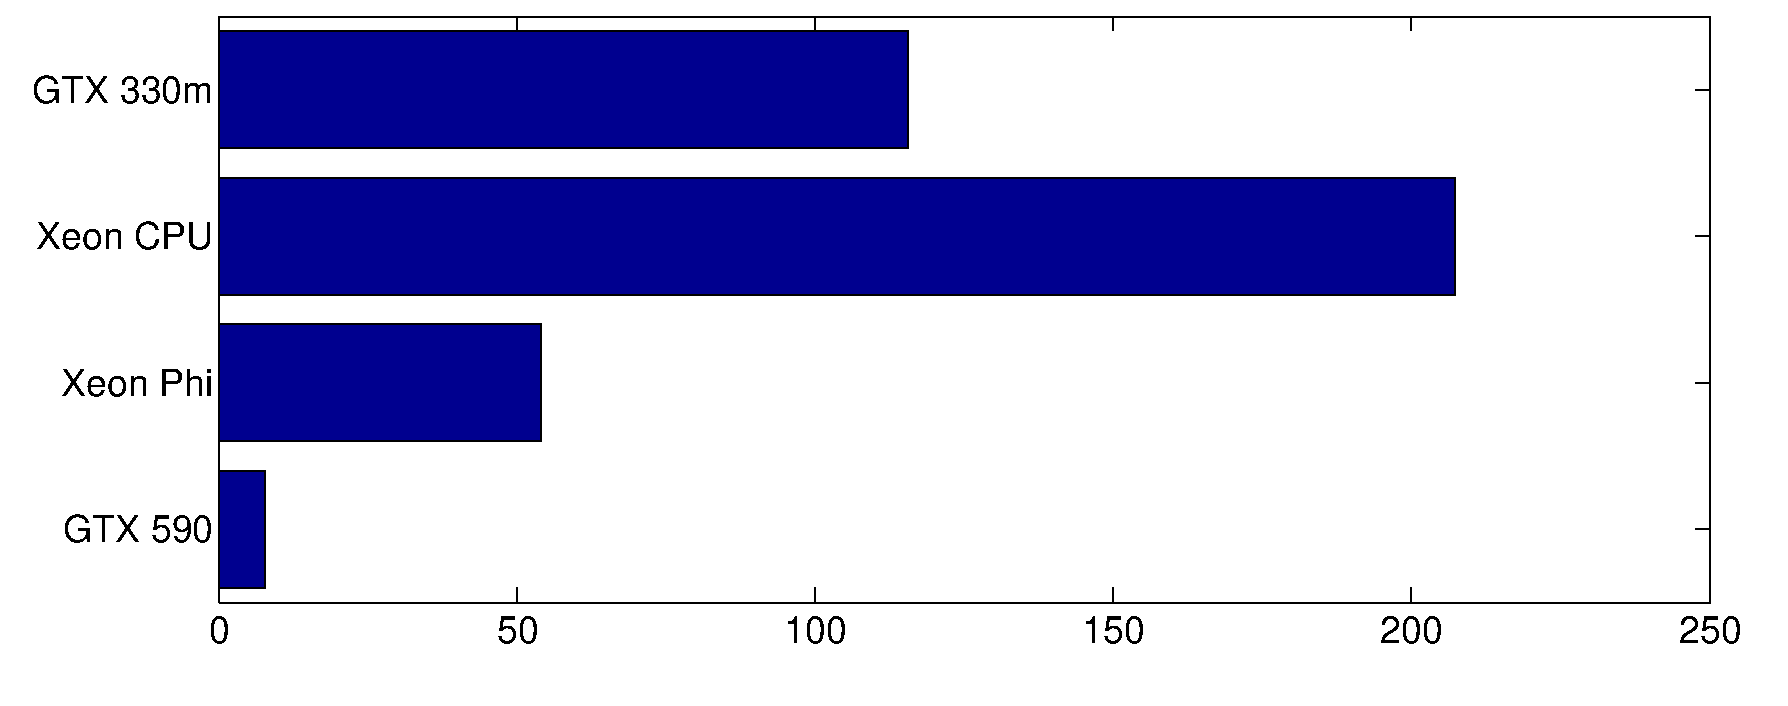
\includegraphics[width=0.9\columnwidth]{figures/eps/runtime.eps}
	  \caption{Egy képre jutó átlagos futási idők [ms]}
	  \label{fig:runtime}
	\end{center}
	\end{figure}
	
	Az eszközök architekturájából fakadó különbségek számszerűsítése végett a futási időt egy compute-unitra és egy órajelre
	fajlagosan számítom.
	\begin{equation}
	T_{fajl} = \frac{T \cdot N_{CU}}{f_{dev}}
	\end{equation}
	ahol $T$ a futási idő $N_{CU}$ az eszköz compute-unit száma és $f_{dev}$ az eszköz órajelének frekvenciája.
	
	\begin{table}[H]
	\footnotesize
	\centering
	
	%\setlength{\extrarowheight}{8pt}
	\begin{tabular}{ l | r | r | r | r}
		 & GTX 330m & Xeon E5-1620 & Xeon PHI & GTX 590\\ \hline
		\texttt{MAX\_COMPUTE\_UNITS} & $6$ & $8$ & $224$ & $16$\\
		\texttt{MAX\_CLOCK\_FREQUENCY} & 1265 & 3000 & 1100 & 1225\\\hline\hline
		Fajlagos futási idő $T_{fajl}$ & $541$ & $539$ & $10750$ & $101$
	\end{tabular}
	
	\caption{Eszközök fajlagos futási idejének összehasonlítása}
	\label{table:results}
	\end{table}	
	
	